\documentclass{standalone}%
\usepackage[T1]{fontenc}%
\usepackage[utf8]{inputenc}%
\usepackage{lmodern}%
\usepackage{textcomp}%
\usepackage{lastpage}%
\usepackage{tikz}%
\usepackage{pgfplots}%
\pgfplotsset{compat=newest}%
%
\usetikzlibrary{positioning}%
%
\begin{document}%
\normalsize%
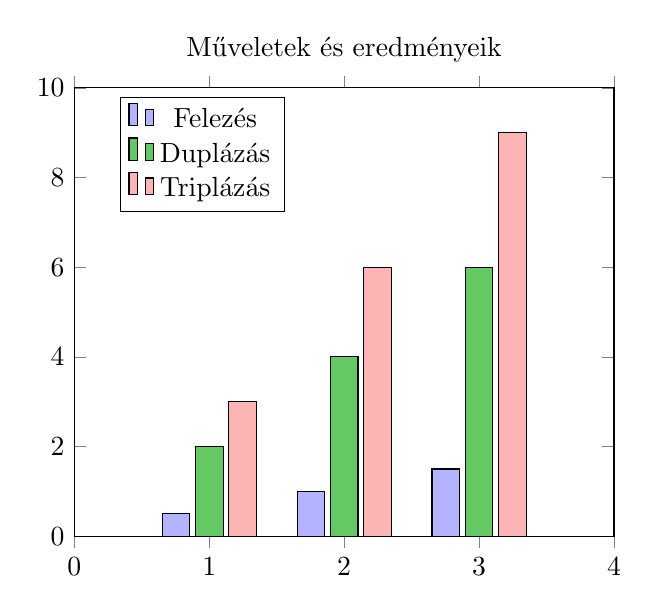
\begin{tikzpicture}%
\definecolor{color1}{RGB}{179, 179, 255}%
\definecolor{color2}{RGB}{100, 200, 100}%
\definecolor{color3}{RGB}{253, 180, 181}%
\begin{axis}[
	ybar,
	name=mygraph,
	title=Műveletek és eredményeik,
	legend style={
		at={
			(0.39, 0.98)
		}
	},
	ymin=0,
	ymax=10,
	xmin=0,
	xmax=4]%
\addplot[fill=color1] coordinates {%
(3.0, 1.5)%
(2.0, 1.0)%
(1.0, 0.5)%
};%
%
%
\addplot[fill=color2] coordinates {%
(3.0, 6.0)%
(2.0, 4.0)%
(1.0, 2.0)%
};%
%
%
\addplot[fill=color3] coordinates {%
(3.0, 9.0)%
(2.0, 6.0)%
(1.0, 3.0)%
};%
%
%
\legend{Felezés, Duplázás, Triplázás}%
\end{axis}%
\end{tikzpicture}%
\end{document}